\documentclass[a4paper]{article}

\usepackage[utf8]{inputenc}    % enables use of utf8 characters in the input file
\usepackage[T1]{fontenc}       % enables proper output of unicode characters such that text can be copy-pasted from the pdf file
\usepackage{hyperref}          % enables pdf index, links for web addresses, intra-document links
\usepackage{a4wide}            % reduces page margins
\usepackage{parskip}           % replaces hanging paragraphs with spacing between paragraphs
\usepackage{times}             % replaces Computer Modern font with something resembling Times
\usepackage{textcomp}          % adds symbols like \textdegree
\usepackage{graphicx}          % enables including graphics
\usepackage{amsmath}           % ams math module
\usepackage{amssymb}           % ams math symbols
\usepackage{mathtools}         % fixes a few quirks with the ams packages

% functions
\DeclareMathOperator{\atan2}{atan2}
\DeclareMathOperator*{\argmin}{argmin}
\DeclareMathOperator*{\argmax}{argmax}

% braces
\newcommand{\xp}[1]{\left(#1\right)}   % parentheses
\newcommand{\xb}[1]{\left[#1\right]}   % brackets
\newcommand{\xc}[1]{\left\{#1\right\}} % curly braces
\newcommand{\xa}[1]{\left|#1\right|}   % absolute value
\newcommand{\xn}[1]{\left\|#1\right\|} % vector norm

% types
\newcommand{\function}[2]{#1 \rightarrow #2}
\newcommand{\R}[1]{\mathbb{R}^{#1}}
\newcommand{\RR}{\mathbb{R}}
\newcommand{\unit}{\xb{0,1}}

% complex terms
\newcommand{\apply}[2]{#1\!\xp{#2}}
\newcommand{\integral}[4]{\int_{#1}^{#2} #3 \; \mathrm{d}#4}
\newcommand{\powerset}[1]{\apply{\mathcal{P}}{#1}}

% continuity
\newcommand{\contp}[1]{\mathrm{C}^{#1}}
\newcommand{\contg}[1]{\mathrm{G}^{#1}}

% vectors
\newcommand{\vectorA}[1]{\begin{pmatrix}#1\end{pmatrix}}
\newcommand{\vectorB}[2]{\begin{pmatrix}#1\\\linebreak{}#2\end{pmatrix}}
\newcommand{\vectorC}[3]{\begin{pmatrix}#1\\\linebreak{}#2\\\linebreak{}#3\end{pmatrix}}
               % some math helper macros

% tells LaTeX to avoid orphan lines at the beginning or end of a page
\clubpenalty = 10000
\widowpenalty = 10000

\title{Optimal Fitting of Planar Curves to Prescribed Constraints}
\author{Julian Asamer, Julian Brunner}
\date{\today}

% TODO: consider splitting some illustrations into multiple figures if there is still space left at the end
% TODO: expand n't contractions
% TODO: check if all quotations are done `like this'
% TODO: maybe extract topical project progress from log
% TODO: consistent use of polynomial, planar, plane, parametric, curve

\begin{document}

	\maketitle

	\begin{abstract}

		\noindent TODO

	\end{abstract}

	\section{Introduction}
	\label{section:introduction}

		These days, vector graphics are widely used in both artistic and industrial design. Artists create illustrations, character designs and even fully animated cartoons using vector graphics software. Vector graphics are also used in industrial design, allowing for the smooth, aerodynamic shapes observed in modern cars and airplanes.

		Raster graphics images (for instance, digital photos and most digitally painted artworks) consist of a finite number of pixels (picture elements) which discretely specify the colors at each point of the image. In contrast, vector graphics designs consist of primitives like curves and surfaces, which describe the shapes present in the design using continuous mathematical functions. This has various advantages over the raster approach, since designs do not suffer from discretization artifacts and can, for instance, be arbitrarily scaled without any loss of quality.

		The scope of this project is restricted to two-dimensional vector graphics, but many ideas can be applied to three-dimensional vector graphics as well. All elements in two-dimensional vector graphics are described in terms of curves, so the design process of curves is the single most important part of two-dimensional vector graphics. Unfortunately, designing curves using the tools available through current vector graphics software can be very frustrating. The artist is often unable to make the curve look the way they want it to. To make matters worse it is often unclear why this is the case, as the software seems to put all the necessary tools into the hands of the designer, yet at times, they somehow don't allow the artist to communicate their intention to the software. Thus, the objective of this project is to identify the exact nature and cause of these inadequacies and then specify and implement curve design tools that do not exhibit them.

		% TODO: make sure introduction does not overlap with start of next section regarding both content and wording
		% TODO: quote raphael levien on usability of Bézier splines
		% TODO: comment on that although there has been some research into better curves (quote MVC curves), it was less focused on usability and hasn't had much impact on actual vector graphics software which continues to almost exclusively use bézier splinse to this day

	% TODO: maybe we don't want to mention G^n and C^n until formally introduced later, doesn't add much value to the usability discussion anyways
	\section{Problem Analysis}
	\label{section:problem_analysis}

		When trying to improve something, it seems advisable to take a step back and thoroughly research the causes of its perceived shortcomings so as to find a way to improve it without making the same or similar mistakes. In the context of curve design tools, this can be achieved by analyzing and modelling the process that people use when designing curves. Once such a model has been obtained, it can be used to propose criteria for good curve design software as well as to analyze potential usability issues with existing tools.

		\subsection{Curve Design Process}
		\label{section:curve_design_process}

			Observing the process that most people seem to go through when designing curves using vector graphics software, the following model appears plausible:
			\begin{enumerate}
				\item obtain the source curve as either a real or a mental image of the curve
				\item extract some properties from the source curve
				\item provide these properties to the software
				\item have the software derive the most likely result curve from these properties
			\end{enumerate}

			Steps 2 to 4 are then repeated on portions of the curve in order to make small adjustments until the result curve is sufficiently similar to the source curve.

			Step 1 is of course independent of any software that may be used by the designer. Step 2 and 3 are strongly influenced by the choice of design tool, in that the software dictates which properties it accepts as specifications for curves (the specification language the software uses). Unless the properties the designer conveyed to the software in step 3 uniquely identify the curve, in step 4, the design tool will have to choose the curve that the user was most likely describing from a possibly infinite set of curves that exhibit the supplied properties. This notion of `most likely' is usually modelled in terms of a fairness measure, fairer curves being regarded as more likely. Fairness ususally encodes intuitive notions such as smoothness using mathematical concepts such as continuity and change in curvature. Here, the software has another opporunity to influence the design process both positively and negatively depending on how the fairness measure is chosen as well as by how good the software is at reliably finding a curve that has a high fairness.

			Note that there may be multiple ways to describe a given curve design tool in terms of this process. Instead of modelling the selection of the most likely curve using some fairness measure, one may also propose an alternate view on the process in which the user implicitly specifies the exact curve they want in the properties they specify. For example, in a curve design tool which takes two points from the user and connects them using a straight line, one may say that the user provides the start and the end point of the curve, and the fairness measure is designed to always select the straight line as the fairest curve. Another way of looking at this process is to say that the user, by supplying \(p_0\) and \(p_1\), specified the coefficients of the linear term \(p_0 + \xp{p_1 - p_0} t\), thus uniquely identifying the desired curve. Modelling the process in such a way that the user supplies only the minimum amount of implicit information, relying on the fairness measure for everything else, is usually closer to reality when analyzing usability of some curve design tool. In a similar fashion, one may consider shortcomings (for instance insufficient continuity) as either shortcomings of the specification language (the language does not allow the user to request \(\contg{2}\) continuity) or as shortcomings of the fairness measure (the fairness measure does not select sufficiently smooth curves).

		\subsection{Usability Criteria for Curve Design Tools}
		\label{section:usability_criteria_curve_design_tools}

			% TODO: properly instroduce description language, how the fairness measure determines semantics but not syntax of that language, etc., figure out when to use description and when to use specification, since they are syntactically identical
			We conclude that the two ways in which curve design software can affect the design process are through the choice of specification language and fairness measure, which we will call the description language. The usability is of course also affected by the software's ability to derive curves from descriptions.

			Ideally, the specification language should be very expressive, yet easy to handle for humans, enabling the user to communicate their intent to the software efficiently. The fairness should capture the intuitive notion of curve smoothness sufficiently well. These goals are competing with the software's ability to derive curves from descriptions reliably and efficiently, a process which becomes increasingly difficult with more expressive specification languages and more complex fairness measures.

			From these considerations, we think that applying the following criteria is a good start for assessing the usability of curve design tools:
			\begin{enumerate}
				\item How efficient is the specification language at describing various curves?
				\item How well can humans `read' the specification language from curves?
				\item How well can humans `speak' the specification language to the software?
				\item How well does the fairness measure capture the intuitive notion of smoothness?
				\item How well can the software derive curves from specifications and a fairness measure?
			\end{enumerate}

		\subsection{Existing Curve Design Tools}
		\label{section:existing_curve_design_tools}

			Using the model of the curve design process as well as the criteria for usability of curve design software that were established in the previous section, various tools available in current vector graphics software can be analyzed.

			\subsubsection{Bézier Splines}
			\label{section:bézier_splines}

				Bézier splines are probably the most widely used type of curve in two-dimensional vector graphics. Bézier splines are defined piecewise using Bézier curves, which are planar parametric curves (functions \(\function{\unit}{\R{2}}\)) realized using polynomials (usually cubic) in Bernstein form. A Bézier curve \(\phi\) of degree \(n\) consists of \(n + 1\) coefficients \(c_i \in \R{2}\). The curve will always go through the first and the last coefficient point (\(\apply{\phi}{0} = c_0, \apply{\phi}{1} = c_n\)) and stay within the convex hull of the coefficient points at all other times. Bézier curves in a Bézier spline are usually pieced together such that the resulting spline is \(\contg{1}\) continuous.

				% TODO: explain velocity
				In existing vector graphics software, Bézier splines are edited by more or less directly modifying the coefficient points of the underlying Bézier curves. In the case of cubic Bézier curves, the first and the last coefficient points represent the curve's start and end points, while the differences between the second and the first as well as the fourth and the third coefficient points are proportional to the velocity of the curve at the start and end points, respectively. In that sense, the user can specify start end end points of the curve, as well as start and end velocities of the curve using the coefficient points. Most vector graphics tools have functions that allow preserving the \(\contg{1}\) continuity of the spline by automatically modifying adjacent coefficient points accordingly. They usually do not ensure \(\contg{2}\) continuity though. Some tools can also modify existing coefficient points in such a way that the curve passes through a point that is chosen by the user without adding more Bézier curves to the spline.

				When applying the model introduced in section \ref{section:curve_design_process} to Bézier spline design tools, there are two possibilities for modelling the fairness measure. One way to view things is to assume that the user, in supplying the four coefficient points of each curve segment, uniquely specifies each segment and thus the entire curve, leaving no room for choosing a curve according to some fairness measure. Since users usually don't think about Bézier splines that way, it is more practical to assume that the user only supplies both point and velocity at the start and end of each curve segment, with a fairness measure designed to always choose the cubic polynomial that is uniquely specified by the given properties as the fairest curve.

				Applying the criteria established in section \ref{section:usability_criteria_curve_design_tools}, we conclude that the design tools for Bézier splines work sufficiently well in terms of humans trying to read and/or speak their specification language (criteria 2 and 3), a skill that can be acquired with some practice. Bézier splines are furthermore very simple to derive from their specification, fulfilling the 5th criterion perfectly. Design tools for Bézier splines have some issues with both the fairness measure (criterion 4) and the expressiveness of the specification language (criterion 1), both of which shall be analyzed in the following paragraphs.

				The issue with the fairness measure is that it always selects the uniquely determined cubic polynomial, thus not guaranteeing \(\contg{2}\) continuity. It is difficult for humans to choose the coefficient points in such a way that \(\contg{2}\) continuity is established, making it hard to create smooth curves if the design software does not support the user in this regard. The problem is aggravated by the fact that curvature discontinuities can be hard to spot and may thus only be discovered much later in the design process, increasing the cost of these mistakes. In case the software allows the user to request \(\contg{2}\) continuous Bézier splines, this sacrifices some degree of freedom for each node, thus restricting the way nodes can be manipulated and in turn possibly forcing the user to place more nodes in order to get the desired result. Placing more nodes leads to some disadvantages that will be discussed further in the paragraphs dealing with specification language expressiveness.

				The specification language used to specify Bézier splines in common design tools is lacking in expressiveness. Specifically, describing curves in terms of their curvature is difficult since curvature may only be specified indirectly through the magnitude of the velocity values (higher velocity resulting in lower curvature). Unfortunately, this is also very dependent on the point and velocity coefficients at the other end of the spline segment. There is also no way to directly specify linearly changing curvature. This makes specifying curvature very tedious, and in case the winding angle of the curve segment is large enough, actually impossible, forcing the designer to use additional nodes in order to get the desired result. Using an excessive number of nodes makes it more tedious and time-consuming for the designer to create and/or modify such curves, since many nodes and handles have to be created or moved in order to change the overall curve. It also sacrifices smoothness, since it's easy to accidently introduce subtle bumps in the curve when using a large number of nodes. Another issue is that without software support for \(\contg{2}\) continuity, using more nodes usually also introduces more points where curvature is not continuous. In cases where the curvature is an important property of the curve (for example the constant curvature of circular arcs, or the linearly changing curvature of spirals), it may be very difficult to specify these properties indirectly using the coefficient points.

				% TODO: consider moving away from the 'source image is traced' samples and use the actual vector graphics leading to those curves
				% TODO: make sure the size of the node visualization is consistent, use visible colors for node visualization, maybe get rid of circles for handles
				\begin{figure}[htb]
					\centering
					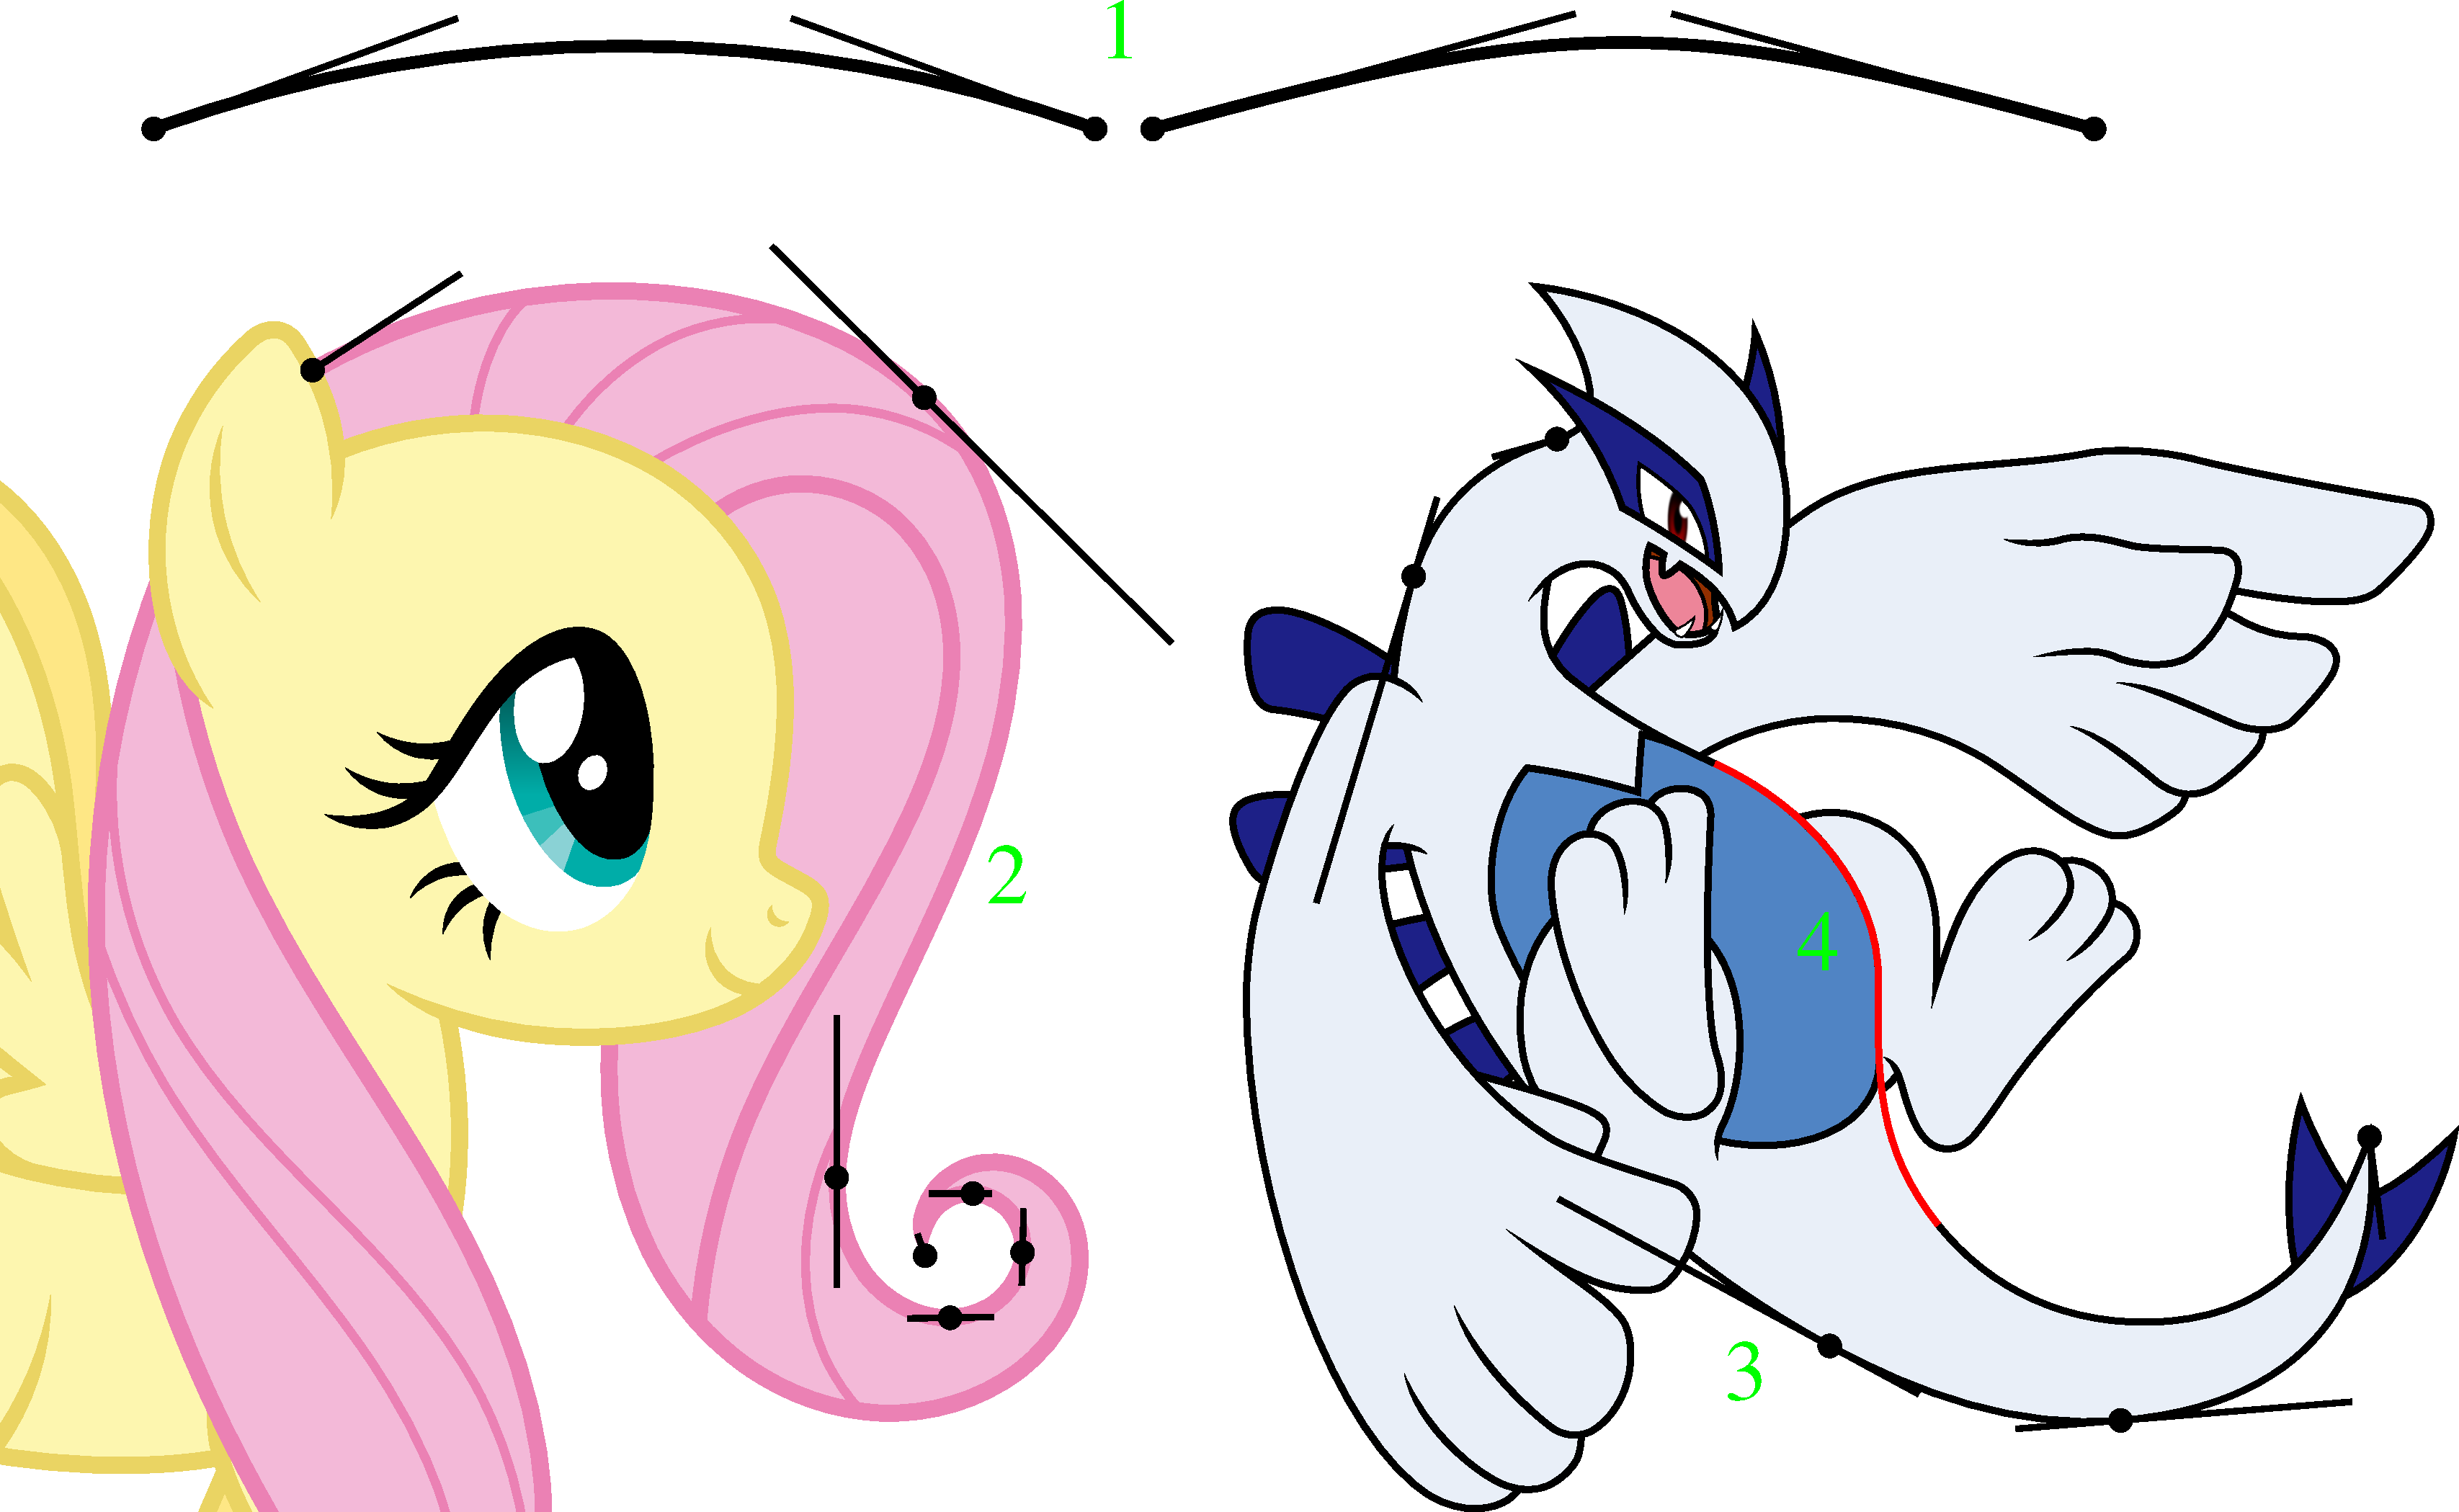
\includegraphics[width=\textwidth]{../resources/usability_bezier.pdf}
					\caption{Usability Analysis of Bézier Splines (left: \cite{Fluttershy}, right: \cite{Lugia})}
					\label{figure:usability_bézier}
				\end{figure}

				% TODO: improve example index numbers (also use font consistent with text)
				Figure \ref{figure:usability_bézier} illustrates some of these issues by showing some examples of Bézier splines as they appear in common design tools. Bézier nodes are displayed as filled dots, while Bézier handles are displayed as circles.

				Example 1 shows two Bézier splines. The left curve is a Bézier spline approximation of a circular arc, exhibiting nearly constant curvature, while the right one is not, going from low curvature to high curvature and back to low curvature. Since the difference can be hard to see, it's easy to make mistakes when trying to approximate circular arcs using Bézier splines.

				Examples 2 and 3 show curves that could be described more efficiently in terms of curvature. Since there is no way to directly specify curvature using Bézier splines, a considerable number of nodes is needed to get close to the desired curve. It may be observed that the spiral in example 2 is not perfect. Creating perfect spirals using Bézier splines is very tedious and would require even more nodes (at least one for every 90\textdegree of winding angle covered). It could be speculated on whether the artist would have opted to use a perfect spiral in this example if they had had the tools to efficiently do so.

				% TODO: consider removing the handle markers to make curvature discontinuity more visible
				Example 4 shows a spline with a curvature discontinuity which went unnoticed by the artist at the time of creation. In fact, this discontinuity would be even less visible if the curve were not vertical at said point, manifesting itself only in a reduced overall smoothness of the curve, without a clear indication of where the problem lies.

			\subsubsection{Spiro Splines}
			\label{section:spiro_splines}

				Spiro splines were added to Inkscape in 2009. Even though they were integrated using path effects and thus have a somewhat cumbersome user interface, they constitute a commendable effort of incorporating results from curve research into vector graphics software, something that has hardly happened this far. More information on Spiro splines can be found in the dissertation of Raphael Levien \cite{Levien2009}.

				Spiro splines consist of parts of the Euler spiral, which is a curve whose curvature changes linearly with the curve's arc length. The user can specify control points through which the software puts an interpolating spline. There is no way to directly specify tangent angle and/or curvature. The splines are guaranteed to have \(\contg{2}\) continuity.

				Again, the model from section \ref{section:curve_design_process} is applied. With Spiro splines, the modelling is fairly straightforward. The user supplies a set of points for which the software computes an interpolating spline. The fairness measure chooses the segments of this spline to be parts of the Euler spiral and makes sure that there is \(\contg{2}\) continuity and no excessive winding.

				We analyze Spiro splines in terms of the criteria presented in section \ref{section:usability_criteria_curve_design_tools}. The specification language of Spiro splines being simply points on the curve, plus the fact that on sufficiently smooth curves, not very many of them being needed, the language is well-suited to be read and spoken by humans (criteria 2 and 3). The fairness measure leads to beautifully smooth curves that are ususally sufficiently close to what a human would expect given the control points (criterion 4). The software is also good and sufficiently quick at constructing these curves (there are some cases where the algorithm fails to find a meaningful curve, but these cases are fairly artificial and can usually be avoided when designing actual curves) and thus fulfills criterion 5 well enough.

				The only real issue lies in the insufficient expressiveness of the specification language. Section \ref{section:bézier_splines} discussed how the lack of ability to specify curvature using common Bézier spline design tools adversively affects usability. Many of the same points apply to Spiro spline design tools, since they allow the user to neither specify tangent angle nor curvature. These properties can only be expressed indirectly, by placing the control points in such a way that the algorithm will create a curve that has the desired properties, resulting in the usability issues described previously, such as requiring many control points to be specified even though the curve could be described much more concisely in terms of tangent angle and/or curvature. This seems especially unfortunate when considering that the spline primitive of Spiro splines, the Euler spiral, would lend itsself excellently to describing circular arcs, spirals and other shapes exhibiting constant or linearly changing curvature. Sometimes, the algorithm can be coaxed into producing the desired curve by placing just a few control points very carefully, resulting in a series of Euler spiral segments that exhibit the wanted properties. Unfortunately, this is rarely practical since it both requires a lot of time to set up and doesn't behave very well when modified. These issues are somewhat alleviated by the guaranteed \(\contg{2}\) continuity together with the general tendency of the algorithm to produce extremely smooth curves even when many control points are involved. That way, when indirectly specifying tangent angle and/or curvature by placing many control points, it's not as easy to accidently create small bumps as with Bézier splines.

				\begin{figure}[htb]
					\centering
					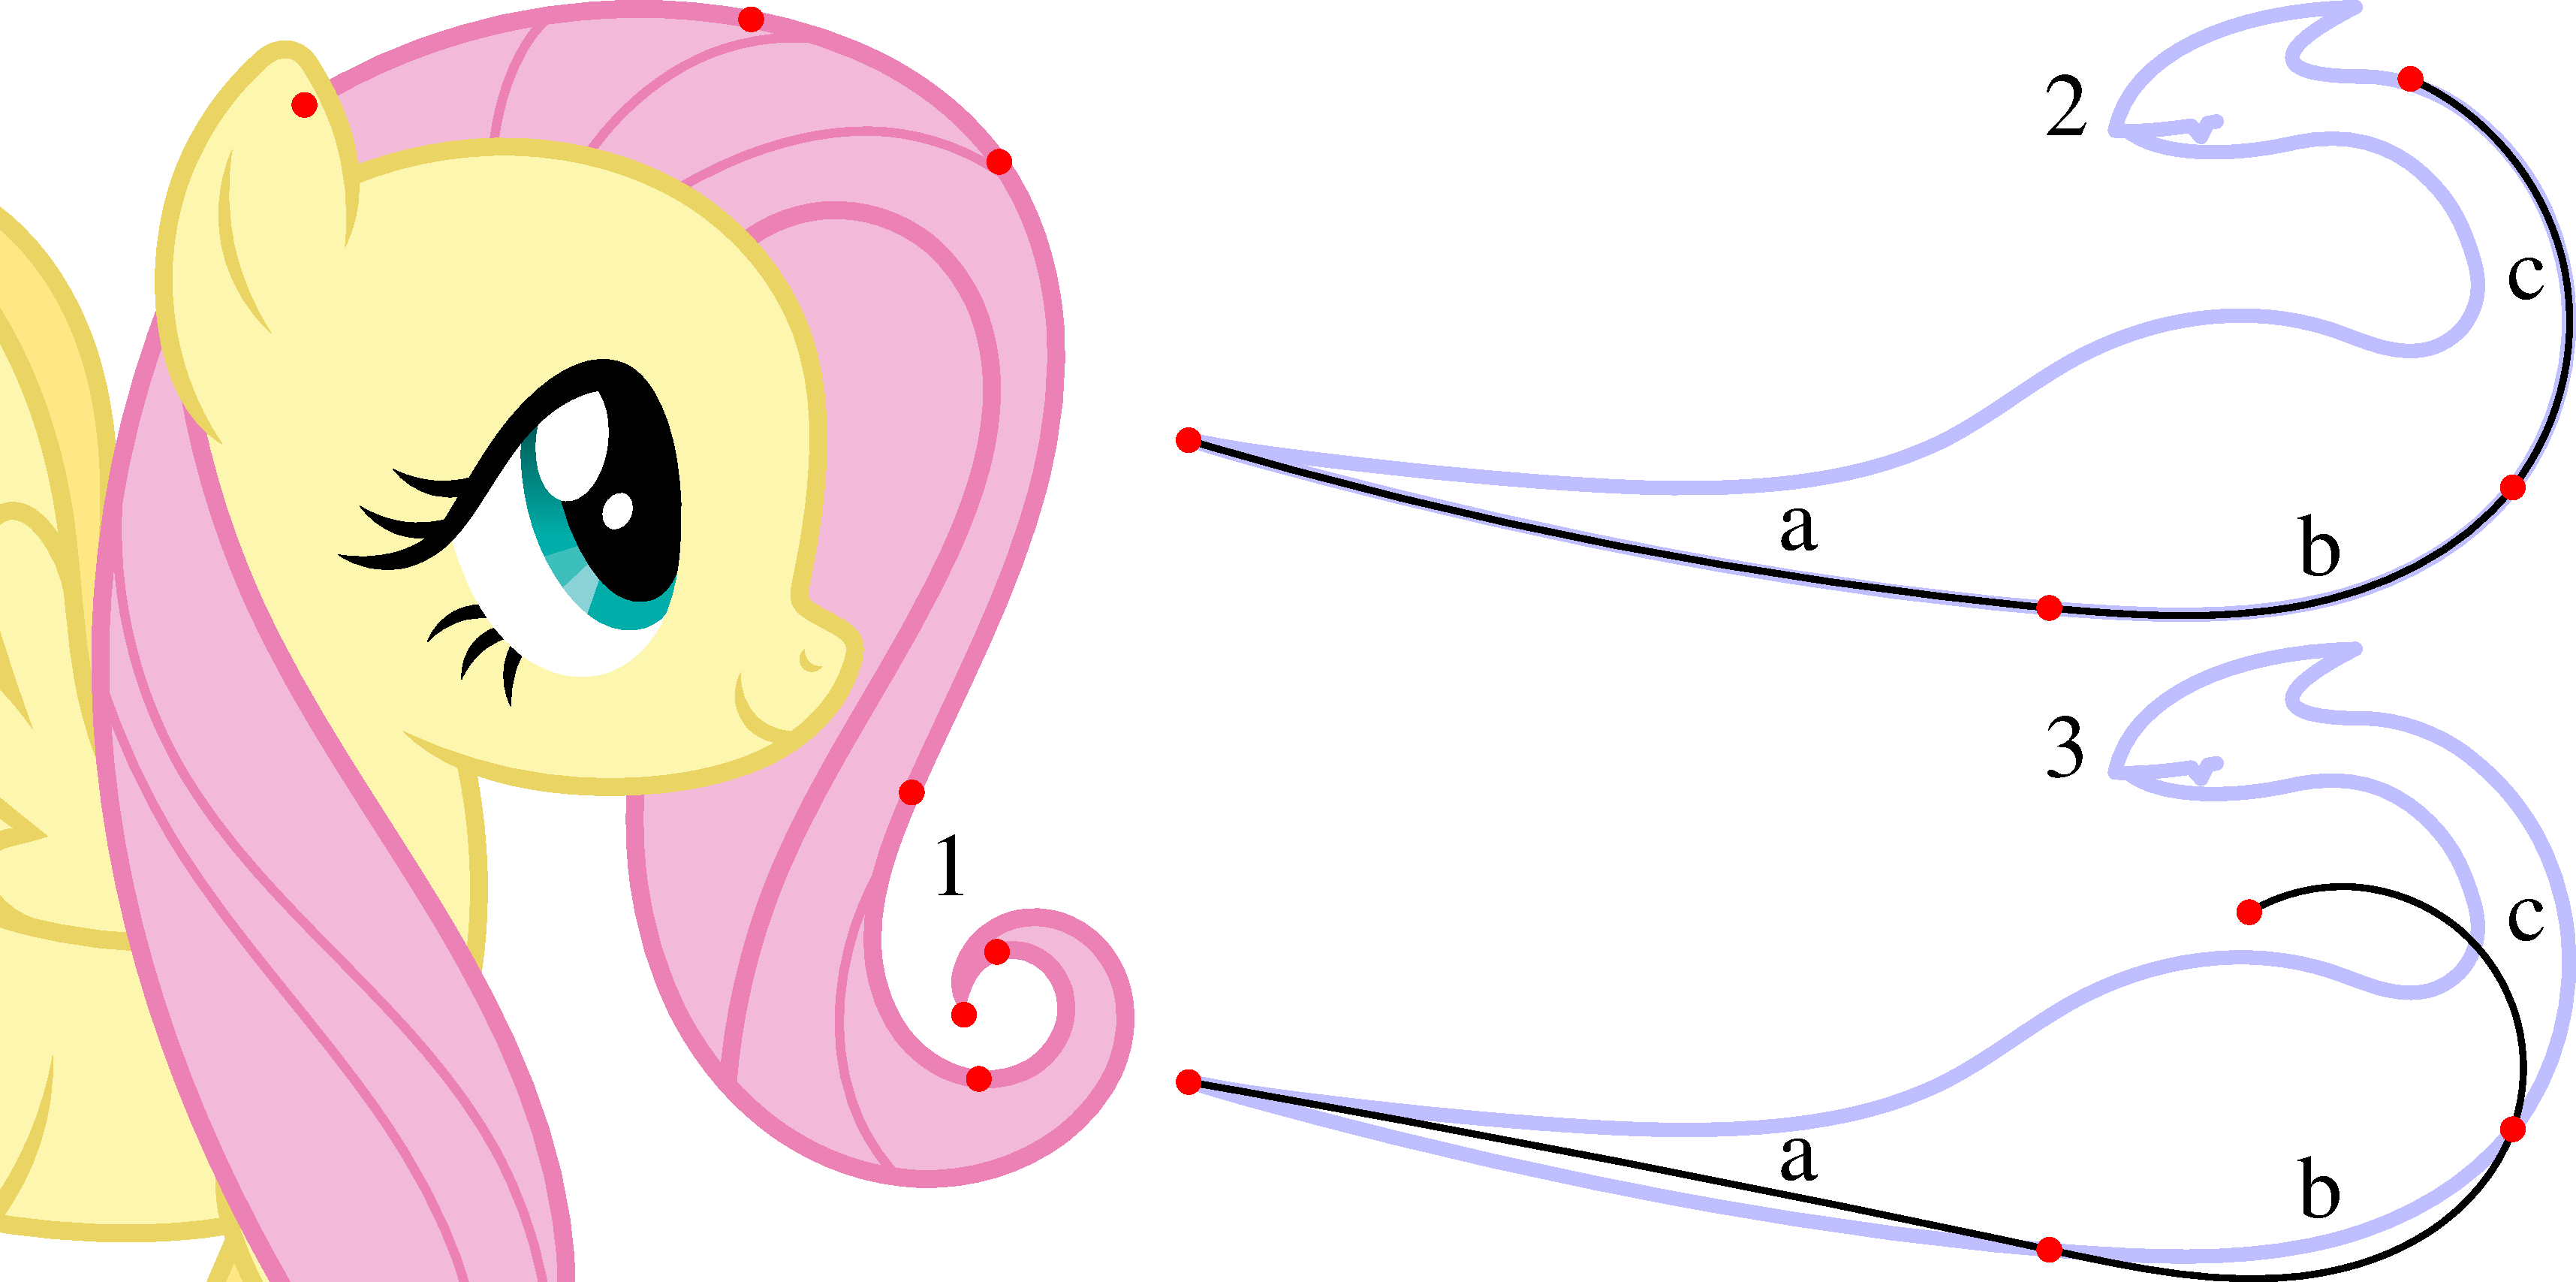
\includegraphics[width=\textwidth]{../resources/usability_spiro.pdf}
					\caption{Usability Analysis of Spiro Splines (left: \cite{Fluttershy}, right: \cite{Lugia})}
					\label{figure:usability_spiro}
				\end{figure}

				% TODO: improve example index numbers
				Figure \ref{figure:usability_spiro} illustrates some of these issues by showing some examples of Spiro splines as they appear in common design tools. Control points are displayed as filled dots.

				Example 1 shows a shape that is in principle well-suited for being represented by parts of the Euler spiral. Unfortunately, describing the curve using Spiro splines still requires many control points. In contrast to the corresponding example in section \ref{section:bézier_splines}, the curve in this example is close to a perfect spiral an thus does not match the source image perfectly. Additional control points would have to be added in order to approximate the imperfect spiral in the source image better.

				Example 2 shows how some shapes can be described using Spiro splines by placing only very few control points. In this case, the shape consists of a circular arc with low curvature (segment a), a segment of linearly increasing curvature (segment b) and finally a circular arc with high curvature (segment c). This shape can be described conveniently using a Spiro spline with just 4 control points.

				Unfortunately, as can be seen in example 3, this scenario does not handle modifications very well. For instance, increasing the curvature of segment c has to be done indirectly by moving a control point. Unfortunately, in this case, this also changes the tangent angle of the curve at that point, such that additional modifications would be needed to correct this. The change also adversely affects segment a, since the curvature there was not specified directly but instead relied on the rather fragile configuration of the 4 control points.

	\section{Definitions}
	\label{section:definitions}

		TODO

		\subsection{Parametric Plane Curves}
		\label{section:parametric_plane_curves}

			In order to be able to reason about curves, a few basic definitions are needed.

			Definitions about vectors in the euclidean plane:
			\begin{align*}
				\overline{\cdot} & : \function{\R{2}}{\R{2}} & \overline{v}      & = \vectorB{-v_2}{v_1}      && \text{orthogonal vector}\\
				\alpha           & : \function{\R{2}}{\RR} & \apply{\alpha}{v} & = \apply{\atan2}{v_2, v_1} && \text{polar coordinate angle}
			\end{align*}

			Definitions about parametric curves:
			\begin{align*}
				\phi    & : \function{\unit}{\R{2}} &                    &                                                && \text{point}\\
				\sigma  & : \function{\unit}{\RR}   & \apply{\sigma}{t}  & = \xn{\apply{\phi'}{t}}                        && \text{speed}\\
				\lambda & : \function{\unit}{\RR}   & \apply{\lambda}{t} & = \integral{0}{t}{\apply{\sigma}{u}}{u}        && \text{covered arc length}\\
				\delta  & : \function{\unit}{\RR}   & \apply{\delta}{t}  & = \apply{\alpha}{\apply{\phi'}{t}}             && \text{direction}\\
				\chi    & : \function{\unit}{\RR}   & \apply{\chi}{t}    & = \frac{\apply{\delta'}{t}}{\apply{\sigma}{t}} && \text{curvature}
			\end{align*}

			Using these definitions, the direction \(\apply{\delta}{t}\) is equal to the tangent angle at the point \(\apply{\phi}{t}\) and the curvature \(\apply{\chi}{t}\) is equal to the inverse of the radius of the osculating circle at the point \(\apply{\phi}{t}\) and it is \(0\) if the curve is locally a straight line at the point \(\apply{\phi}{t}\).

		\subsection{Continuity}
		\label{section:continuity}

			% TODO: introduce parametric and geometric continuity

	\section{Proposed Solution}
	\label{section:proposed_solution}

		Having analyzed the usability aspect of curve design tools in \ref{section:problem_analysis}, it's time to think about how to properly address their current issues. In the following sections, we propose both an abstract approach for designing usability-oriented curve design tools, as well as our specific ideas for developing a piece of software using this approach.
          
		\subsection{Description-Based Curves}
		\label{section:description-based_curves}

			Seeing how the description language almost completely determine all usability aspects of the resulting curve design tool, it seems unwise to choose them based on low-level mathematical aspects of the curve as is the case with Bézier splines. Spiro splines are much better in that a lot of effort was put into the fairness measure. Unfortunately, the project has set out to solve the problem of constructing interpolating splines, thereby committing to a very restricted specification language right from the start.

			We think that in order to get the best usability, using a good specification language which does not rely on implementation details has to be the top priority. Together with a good fairness measure, it forms a description language that, if it allows for reliable and efficient derivation of curves, will then lead to usable curve design tools. Since it is not immediately clear which description language is the best, the first step is to move away from the traditional explicit curve construction, and instead use a process that enables the creation of curves based on descriptions.

			\begin{figure}[htb]
				\centering
				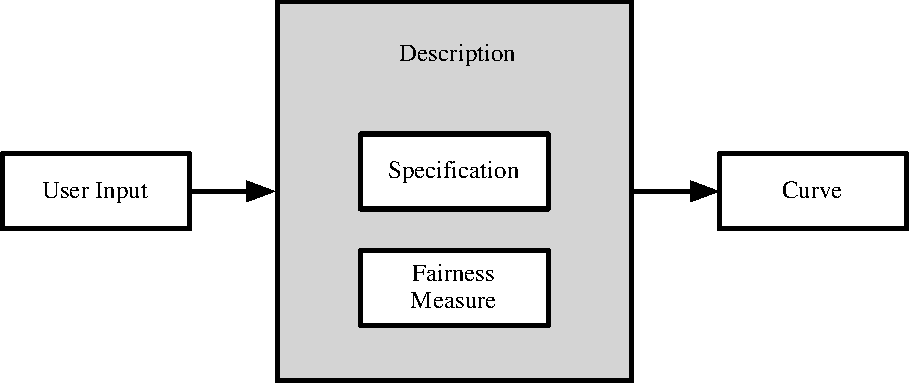
\includegraphics[width=\textwidth]{../resources/description-based_curves.pdf}
				\caption{Description-Based Curves}
				\label{figure:description-based_curves}
			\end{figure}

			Figure \ref{figure:description-based_curves} shows such a process. Note that this approach doesn't give any specifics yet, since the previous usability analysis didn't give a complete answer as to what the optimal curve design tool looks like. It has yet to be determined what the description language should be, as well as how to derive curves from these descriptions.

		\subsection{Description Language}
		\label{section:description_language}
			
			After establishing the general approach to curve design tools in section \ref{section:description-based_curves}, it's time to decide on the specifics in order to create an instance of this model. The first step is to choose a description language, consisting of both a specification language and a fairness measure.

			% TODO: talk about insensitivity of the human visual system to properties beyond the second derivative in both sections, build everything on that premise

			\subsubsection{Specification Language}
			\label{section:specification_language}

				The specification language we propose uses differential geometric properties of curves and is thus decoupled from specifics of the underlying curve model, hopefully leading to a specification language that is easier to learn and use. The human visual system seems to be fairly insensitive to curve properties beyond the second derivative, so the specification language will focus on the properties point, direction and curvature as defined in \ref{section:parametric_plane_curves}. In order to provide the maximum flexibility, the specification language should allow to specify any combination of these three properties at any number of positions on the curve.

				With point specifications, it's sometimes enough to require the curve to go through all of them in order, although sometimes, this will lead to undesirable results. Even with the curve preserving the order in which the points are visited, it is unspecified how much arc length the curve will spend between each pair of points. When specifying direction and/or curvature without an associated point, it becomes a necessity to associate this specification with some kind of positional information in order to anchor it to some point on the curve. If this was not done, the specification could move freely along the curve and would thus behave very unpredictably. We thus chose to associate each combination of point, direction and curvature with a position on the curve.

				With that in mind, it is now possible to abandon this notion of a combination of point, direction and curvature and instead talk about specification items, a specification item being either a positioned point, a positioned direction or a positioned curvature. A combination of point and curvature at some position thus splits up into a point specification item at this position and a curvature specification item at the same position.

				An obvious choice for specifying a position on a curve would be by giving a parameter value for the underlying parametric curve. However, this would violate our design idea of using differential geometric properties of curves. A way of specifying a position on a curve that is independent from its parametrization is the arc length of the curve. Instead of directly using the arc length to give the positions of specification items, we chose to specify positions as fractions of the total arc length of the curve. This way, the position of a specification item relative to the start and end points of the curve is independent of the total arc length of the curve.

				With this setup, it seems advisable to also include the curve's total arc length in the specification. This way, one can specify curves that don't have any specification items associated to their start and end points. Also, with unspecified curve length, changing any specification item may inadvertently change the curve's total arc length, thus possibly adversely affecting other parts of the curve whose specification item positions are given as a fraction of the curve's total arc length.

				Thus, the final specification language is as follows:
				\begin{equation*}
					\begin{alignedat}{2}
						& \mathrm{Positions}          && = \unit\\
						& \mathrm{Points}             && = \R{2}\\
						& \mathrm{Directions}         && = \RR\\
						& \mathrm{Curvatures}         && = \RR\\
						& \mathrm{SpecificationItems} && = \mathrm{Positions} \times \left(\mathrm{Points} \cup \mathrm{Directions} \cup \mathrm{Curvatures}\right)\\
						& \mathrm{CurveLengths}       && = \RR\\
						& \mathrm{Specifications}     && = \powerset{\mathrm{SpecificationItems}} \times \mathrm{CurveLengths}
					\end{alignedat}
				\end{equation*}

			\subsubsection{Fairness Measure}
			\label{section:fairness_measure}

				% TODO: add citations
				% TODO: make clear that these terms are to be minimized
				% TODO: explain how the MVC fairness reduces unnecessary inflection points, etc.

				Many different fairness measures for plane curves have been proposed throughout history. Most of them set out to emulate the behavior of mechanical splines made from wood or steel, which were used for industrial design before the advent of computer aided design. The most direct approach of this type uses mechanics to derive a term for the energy in an idealized bent steel band, arriving at the following functional describing the minimum energy curve (MEC):
				\begin{equation*}
					\integral{0}{1}{\apply{\chi}{t}^2}{t}
				\end{equation*}
				While this approach is a good idealization of the mechanical spline, it has some disadvantages when used for curve design. For instance, it will not yield a circular arc when constrained by co-circular points.

				Thus, there has also been some research into fairness measures whose design is more directly motivated by the human perception of smoothness in plane curves. One such approach is that of the minimum variation curve (MVC), whose functional is given below:
				\begin{equation*}
					\integral{0}{1}{\apply{\chi'}{t}^2}{t}
				\end{equation*}
				Minimum variation curves capture the intuitive notion of smoothness very well. The functional will put straight lines through points that are co-linear and circular arcs through points that are co-circular when otherwise unconstrained. When constraints cause different points on the curve to have different curvatures, the functional will prefer linearly changing curvture, since that will make the derivation of the curvature a constant and thereby minimize the integral over the square of the derivative of the curvature. Because of these appealing properties, the MVC fairness measure was chosen.

		\subsection{Curve Derivation}
		\label{section:curve_derivation}

			Implementing the approach presented in section \ref{section:description-based_curves} requires a way of turning descriptions into actual curves. We chose to use nonlinear optimization on polynomial splines in order to achieve this goal.

			Nonlinear optimization allowed us to stay relatively flexible with respect to the description language and enabled us to experiment with different specification languages and fairness measures, assessing their usability before settling on the choices presented in section \ref{section:description_language}.

			Polynomial parametric curves were chosen since they are mathematically simple, very flexible through the choice of their degree, and are well-suited to approximate a variety of smooth curves. We opted to use polynomial splines since they allow approximating more complex curves without involving polynomials of excessively high degree, which are known to have poor stability.

			\subsubsection{Optimization Problem}
			\label{section:optimization_problem}

				Nonlinear optimization problems are usually expressed using an objective function \(f : \function{\R{n}}{\RR}\), a constraint function \(g : \function{\R{n}}{\R{m}}\) and constraint bounds \(g_l, g_u \in \R{m}\). The optimization problem is then given by the task of finding an \(x^* \in \R{n}\) such that:
				\begin{equation*}
					\begin{gathered}
						x^* = \argmin_{x \in \R{n}} \apply{f}{x}\\
						g_l \leq \apply{g}{x^*} \leq g_u
					\end{gathered}
				\end{equation*}
				This allows expression of a variety of optimization goals. The ones that are important for us are zero-error constraints (using the constraint function and bounds to specify that an error term is zero), upper bounds on errors (using the constraint function and bounds to specify an upper bound for an error term) and minimization goals (using the objective function to express that an error term should be minimized).

				In the following, we will describe how nonlinear optimization can be used for building polynomial splines based on descriptions in the description language established in section \ref{section:description_language}.

				% TODO: proper explanation of how segments are put together to a spline (wrt. parameter t)
				When using polynomial splines, the optimization domain is a vector consisting of all the coefficients of all the polynomials that make up the spline. Let \(m\) be the number of segments. In the following, we will denote the vector of coefficients of the \(i\)th polynomial by \(c_i\), and the vector of all coefficients by \(c\). The functions defined in section \ref{section:parametric_plane_curves} are used with subscripts (\(\apply{\phi_c}{t}\)) to indicate their dependence on the coefficient vector \(c\). They may also be used with an indexed coefficient vector (\(\apply{\phi_{c_i}}{t}\)) when referring to the \(i\)th segment of the spline.

				Let \(n\) be the number of specification items, with the \(i\)th item being at position \(\hat{t}_i\). If the \(i\)th item is a point specification, the point is denoted \(\hat{\phi}_i\), if it is a direction specification, the direction is denoted \(\hat{\delta}_i\) and if it is a curvature specification, the curvature is doneted \(\hat{\chi}_i\). The specified total arc length for the curve is denoted \(\hat{\lambda}\).

			\subsubsection{Constant Speed}
			\label{section:constant_speed}

				Since we chose to give the position of a specification item as a fraction of the curve's total arc length, we need the function mapping the covered arc length to the corresponding parameter values in order to state the optimization goals for the specification items. Unfortunately, this function is not very well-suited to be used as a term in a smooth opimization problem even for simple curves like polynomials. Also, since the function isn't fixed and varies with the coefficients, there is no way to tell on which segment each specification item will end up, something that is also difficult to state in a smooth optimization problem. We also need to state the specification of the total arc length of the curve as an optimization goal, which may be difficult if the the covered arc length function is hard to express. In order to address these problems, the following error term is used:
				\begin{equation*}
					\apply{e_a}{c} = \max_{t \in \unit} \xa{\apply{\sigma_c}{t} - \hat{\lambda}}
				\end{equation*}
				For polynomial splines with sufficient degree and segment count, this term will be brought close to zero in the optimization, making the speed approximately constant with value \(\hat{\lambda}\). This, in turn, makes the covered arc length function approximately linear (\(\apply{\lambda_c}{t} \approx \hat{\lambda}t\)) which causes the inverse of the covered arc length function \(\lambda_c^{-1}\) to be approximately linear as well, facilitating the simple statement of the optimization goals for the specification items as well as fixing the segment for each specification item. It also causes the total arc length of the curve to be approximately equal to \(\hat{\lambda}\), as requested by the specification.

				Since this goal can only be fulfilled approximately by polynomial curves, it is impossible to use the error term given above in a zero-error constraint. It could however be used in both an upper bound on errors and in a minimization goal. Both approaches were implemented and tested, with the latter yielding a more stable optimization process.

				The error term given above is not well-suited for smooth optimization because it incorporates finding a maximum. Since the optimization problem will allow the original error term to be brought close to zero, we can approximate it using the following error term:
				\begin{equation*}
					\apply{e_b}{c} = \integral{0}{1}{\xp{\apply{\sigma_c}{t} - \hat{\lambda}}^2}{t}
				\end{equation*}
				This term is then finally used as part of the objective function, thus making it a minimization goal.

			\subsubsection{Continuity Connections}
			\label{section:continuity_connections}

				As mentioned in section \ref{section:description_language}, we are not concerned with properties beyond the second derivative of the curve. Thus, we will only require \(\contg{2}\) continuity for the whole spline. While the polynomial curve segments are smooth (\(\contp{\infty}\) continuity), the resulting spline in general is not. The segments have to be pieced together in such a way as to ensure a certain degree of smoothness. Thus, to ensure \(\contg{2}\) continuity for the whole curve, it is sufficient to ensure \(\contg{2}\) continuity at the segment connection points. To do this, the following error terms are added for each connection point (\(0 \leq i \leq m - 1\)):
				\begin{equation*}
					\begin{aligned}
						\apply{e_c}{c} & = \apply{\phi_{c_i}}{1} - \apply{\phi_{c_{i+1}}}{0}\\
						\apply{e_d}{c} & = \apply{\phi'_{c_i}}{1} - \apply{\phi'_{c_{i+1}}}{0}\\
						\apply{e_e}{c} & = \apply{\phi''_{c_i}}{1} - \apply{\phi''_{c_{i+1}}}{0}
					\end{aligned}
				\end{equation*}
				These error terms being zero implies \(\contp{2}\) continuity. However, since the constant speed requirement introduced in the previous paragraph collapses \(\contp{2}\) continuity and \(\contg{2}\) continuity, this is equivalent to the original requirement of ensuring only \(\contg{2}\) continuity, yet better suited for optimization. 

				Since it is not acceptable for the curve segments to not touch, have sharp corners or curvature discontinuities, the error terms above are added as zero-error constraints.

			\subsubsection{Specification Items}
			\label{section:specification_items}

				Having taken care of the somewhat technical details arising from using polynomial splines, it's time to state the error terms for the specification items. For each specification item (\(0 \leq i \leq n\)), we add one of the following error terms, depending on the type of the specification item:
				\begin{equation*}
					\begin{aligned}
						\apply{e_f}{c} & = \apply{\phi_c}{\hat{t}_i} - \hat{\phi}_i\\
						\apply{e_g}{c} & = \apply{\delta_c}{\hat{t}_i} - \hat{\delta}_i\\
						\apply{e_h}{c} & = \apply{\chi_c}{\hat{t}_i} - \hat{\chi}_i
					\end{aligned}
				\end{equation*}

				The user usually wants to specify exact curve behavior rather than indirectly influencing its properties, so these error terms are also added as zero-error constraints.

			\subsubsection{Fairness Error}
			\label{section:fairness_error}

				Finally, the error term for the MVC fairness measure as defined in section \ref{section:fairness_measure} is used:
				\begin{equation*}
					\apply{e_i}{c} = \integral{0}{1}{\apply{\chi'_c}{t}^2}{t}
				\end{equation*}

				It's clear that in many cases, this error term will not be zero, and in fact, may be arbitrarily large. Thus, it is not suitable to be constrained to zero or bounded error and has to be stated as a minimization goal.

			\subsubsection{Complete Formalization}
			\label{section:complete_formalization}

				% give objective and constraints function
				% check code to see if anything was left out

	\section{Implementation}

		% choice of platform
		%   C#: platform independent, high-level, possibility to interface with native code, familarity, good UI frameworks (GTK#)
		%   ipopt
		%   casadi
		%   link to googlecode page
		% numeric optimization
		%   trapezoid sum to approximate integrals
		%   formalization of model using symbolic functions in casadi
		%   optimization using ipopt
		%   caching
		%   keeping track of disambiguation information
		%   input is a set of specifications, disambiguation, etc.
		%   result is a curve whose segmentation is no longer visible
		% user interface (include screenshots)
		%   goal: proof of concept
		%   interacts with numeric optimizer
		%   specify any combination of point, direction and curvature at positions on the curve
		%   change position of a specification
		%     in case of pointspecifications optionally moving the point along the curve accordingly
		%   insert/remove curve length at or between specifications
		%   displays deviation from set velocity, such that the user knows when a segment is over-stretched, or where the curve degree/segment count is too low
		%   loading/saving of documents
		%     specification can be serialized from/to XML

	\section{Evaluation}

		% were the goals met? (TODO: systematic approach for describing expressiveness and new features)
		%   controlling length is actually a very nice thing to have
		%     a good way to control circular arcs in terms of radius (fluttershy's ear, mouth)
		%     a good way to pull curves in place when they don't have direction specifications
		%   fluttershy's mane
		%     spirals done this way are guaranteed to be smooth and not have any unintentional bumps
		%     comparison with bézier
		%       source image is in flash, already made of bézier splines, easy to trace
		%       still many more nodes needed
		%       hard to get actual, perfect spirals right
		%       curvature incontinuities, small bumps
		%     somewhat hampered by poor performance and optimization stability issues, concept seems very powerful though
		%   some curves are more easily described in terms of curvature than points and/or direction
		% problems
		%   local optima
		%   bad stability, infeasible for numeric optimization
		%   performance
		%     possible improvements
		%       make sure substitutions only happen where and when necessary
		%       cache partially instantiated IpoptProblem? such that fewer substitutions have to happen when changing a single specification
		%       use better linear solver with ipopt
		%       properly configure ipopt options
		%       adaptive segment density
		%       adaptive velocity/fairness trapezoid sum

		% demonstrate euler spirals and bézier curves being embedded
		%   minimization of normal jerk squares prefers linear change in curvature
		% take examples from demo
		% revisit examples made when analyzing Bézier splines and Spiro splines
		% a bézier node comes with 2 handles, making it 3 points, or 6 scalar values that are specified, compared to 2 scalars for a DC specification

	\section{Conclusion}

		% distinguish between further research work and turning the project into practical software)	
		% further possibilities to instantiate overall structure (different and/or combined spline primitives, constructive instead of optimization approach)
		% adaptive line segments, adaptive bézier approximation
		% steps that are necessary to turn this project into a useful application
		%   make absolutely sure the concept works by testing it with actual users
		%   performance improvements
		%   inkscape plugin
		% possibility to have curves without fixed length? could be useful for curves which only have specifications at the start and/or end of the curve
		% investigate into the calculus of variations and whether there may be a possibility to construct MVC curves based on our specification format, once the format itsself has proven to be useful

	\begin{thebibliography}{}

		\bibitem{Levien2009}
			\emph{From Spiral to Spline: Optimal Techniques in Interactive Curve Design}\\
			Raphael Linus Levien\\
			University of California, Berkeley, Fall 2009

		\bibitem{Fluttershy}
			\emph{Fluttershy}\\
			Hasbro, Inc.\\
			My Little Pony: Friendship is Magic, 2010

		\bibitem{Lugia}
			\emph{Lugia}\\
			Nintendo Co., Ltd.\\
			Pokémon, 1999

	\end{thebibliography}

\end{document}
